\subsection{Target}
The main target of the project are people that have fear of speaking in public. This kind of fear can be categorized as part of social phobia, i.e. "persistent fears of situations involving social interaction or social performance or situations in which there is the potential for scrutiny by others"\cite{model}.

\subsection{Context and Needs addressed}
"In social/evaluative situations, the primary threat stimulus is an audience and the primary threatening outcome is negative evaluation from the audience"\cite{model}.
This means that the idea of being evaluated by the audience is enough to start a loop that keeps fuelling the anxiety of the subject as shown in figure \ref{fig:model}.
\begin{figure}[H]
	\centering
	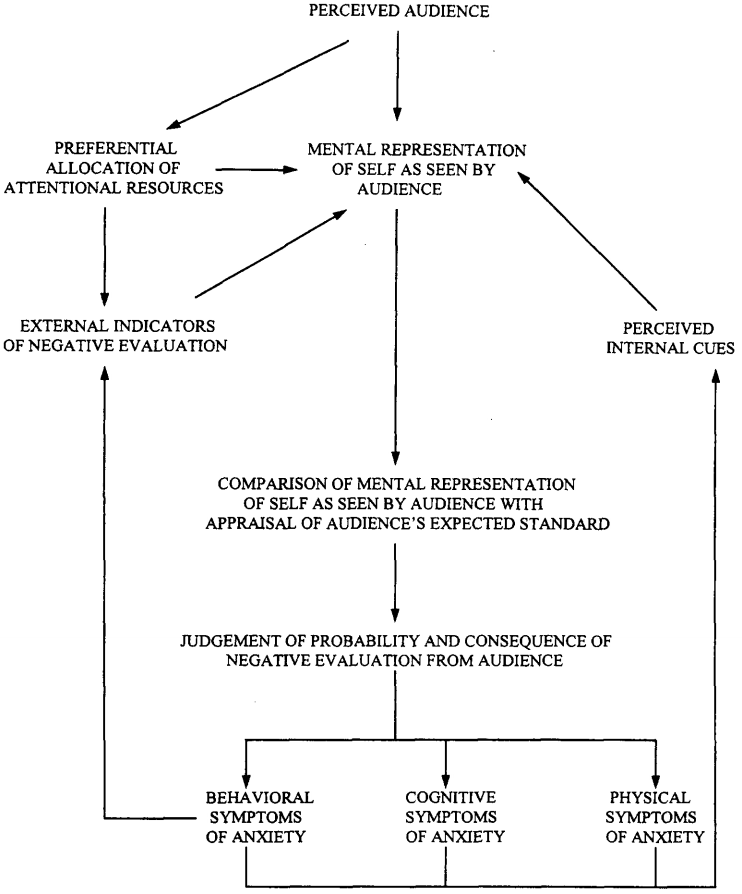
\includegraphics[scale=0.55]{Model}
	\caption{A model of the generation and maintenance of anxiety in social/evaluative situations\cite{model}.}\label{fig:model}
\end{figure}

Knowing this, the needs that were identified are:
\begin{itemize}
	\item Have more confidence around people during the speech
	\item Listen to the speech after the performance
\end{itemize}

\subsection{Goals}
\begin{itemize}
	\item Improve the ability to speak in public
	\item Allow the subject to be less anxious before and during the speech
\end{itemize}

\subsection{Requirements}

\begin{itemize}
	\item The applications should provide an environment where the subject can try his/her speech in front of a virtual audience.
	\item The application should progressively change the number of people that the user can see in the audience based on his/her state of mind.
	\item The application must stop the test in case the subject doesn't feel well.
	\item The application should reward the user at the end of his/her speech.
	\item The application should record the speech and play it if needed.
\end{itemize}

\subsection{Constraints}
\subsubsection{Base}
\begin{itemize}
	\item HMD;
	\item A smartphone running Android Jellybean or higher (4.1.x+);
	\item Empatica E4;
	\item Microphone;
	\item Headphones;
	\item Comfortable place where the user can sit down and rest the arm;
	\item An internet connection.
\end{itemize}

\subsubsection{Pc Client}
\begin{itemize}
	\item A pc (Windows 7 or higher) with Visual C++ Redistributable Package installed;
	\item Bluegiga Bluetooth Smart Dongle;
	\item E4 Streaming Server installed.
\end{itemize}

\subsubsection{Android Client}
\begin{itemize}
	\item A smartphone running Android.
\end{itemize}






